\section{Benchmark Queries}
\label{sec:benchmark}

\subsection{Q1: LCA}
This query is to compute the least common ancestor (LCA) of two 
academic papers. An ancestor of paper $p$ is transitively defined as:

\begin{enumerate}
    \item Any paper that $p$ cites is an ancestor of $p$
    \item Any paper that $p$'s ancestor cites is an ancestor of $p$
\end{enumerate} 

Given two paper $p_1$ and $p_2$, if their sets of ancestors are 
$a(p_1)$ and $a(p_2)$, their common ancestors are 
$a(p_1) \cap a(p_2)$. We define the distance from a common ancestor
as $d(a_1, p_1, p_2) = max(dist(a_1, p_1), dist(a_1, p_2))$, where 
$dist(a_1, p_1)$ is the minimum number of citation hops from $a_1$ to 
$p_1$. Then we can define a total ordering among the common ancestors
of $p_1$ and $p_2$ as, if $a_i, a_j \in a(p_1) \cap a(p_2)$, 
$a_i \prec a_j$ if and only if.

\begin{enumerate}
    \item $d(a_i, p_1, p_2) < d(a_j, p_1, p_2)$.
    \item $d(a_i, p_1, p_2) = d(a_j, p_1, p_2)$ and the year when $a_i$
    published $year(a_i)$ is earlier than $a_j$'s $year(a_j)$.
    \item if $d(a_i, p_1, p_2) = d(a_j, p_1, p_2)$ and $year(a_i) = year(a_j)$, $a_i$'s paper id is a smaller number than $a_j$'s.
\end{enumerate}

\subsection{Q2: K-Core}

The query is to compute the $k$-core (or $k$-degenerate graph) 
of an undirected graph. It is firstly defined by Paul Erd\H{o}s 
and Hajnal as color number \cite{ErdosH66}. 
$k$-core is an important structural property
and has been studied extensively in network analytics 
\cite{Alvarez-HamelinDBV05NIPS, ChengKCO11ICDE}.

A $k$-core of a graph $G$ is a maximal induced subgraph of $G$ in which all
vertices have degree at least $k$ in the subgraph. 
Figure~\ref{fig:k-core_example} shows $1 \ldots 3$-cores of a graph. 

\begin{figure}[t]
    \centering
    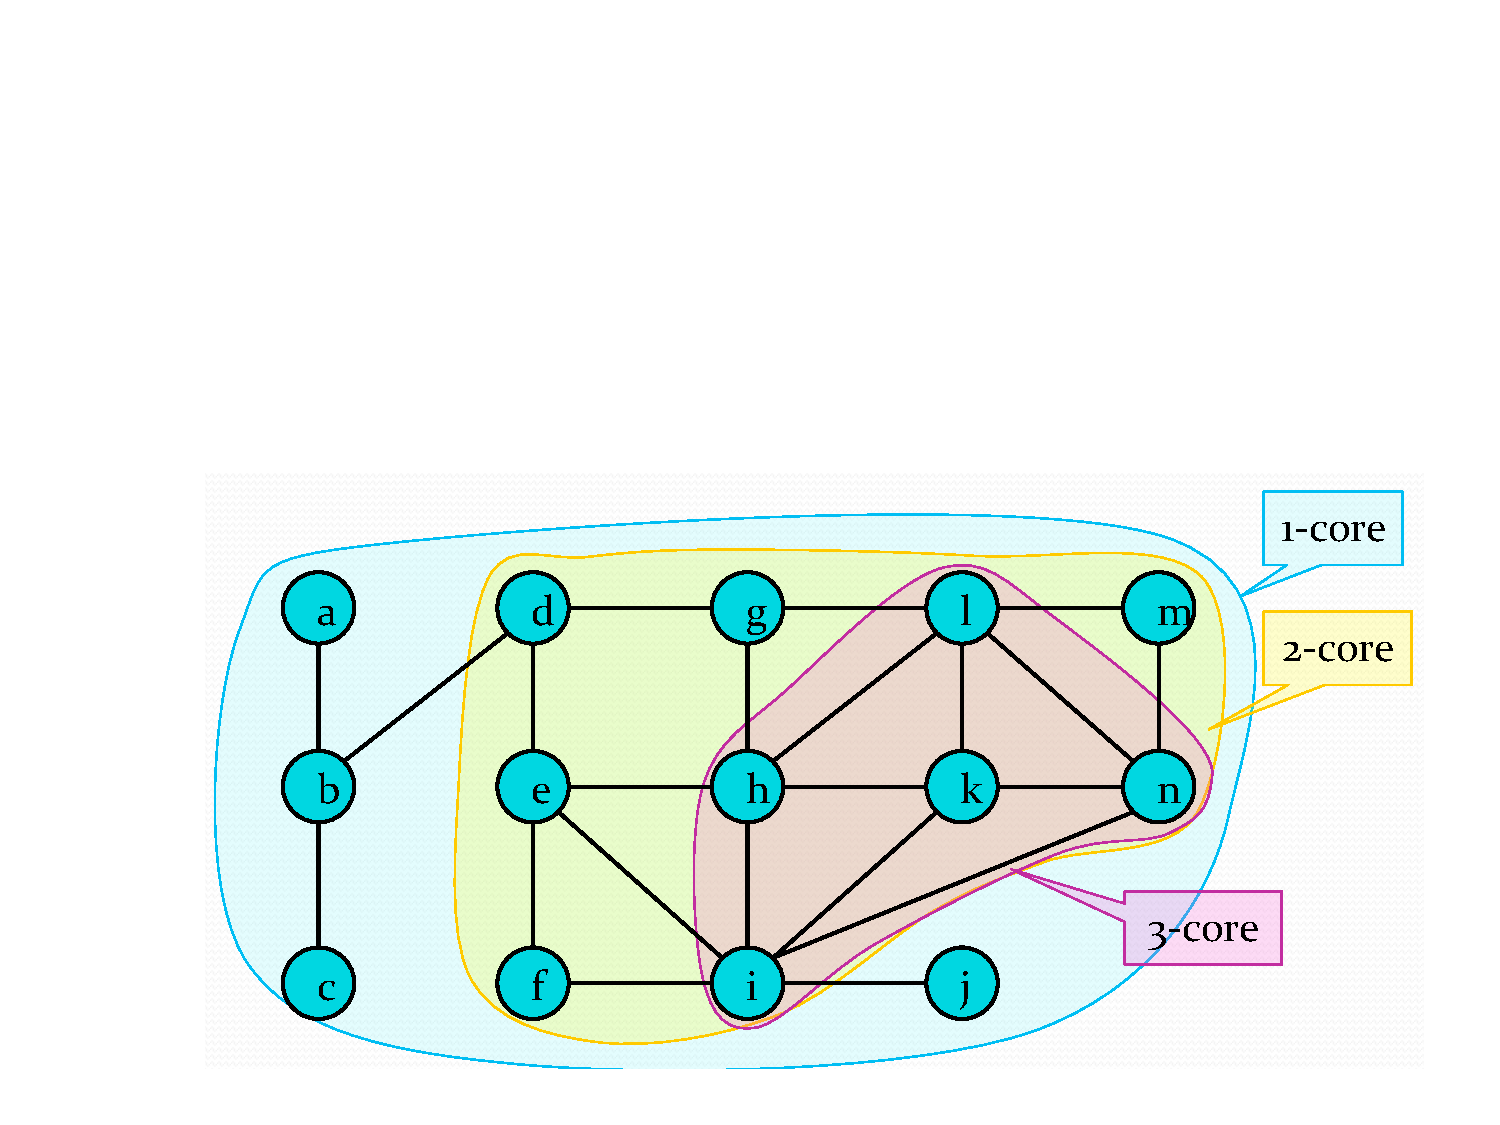
\includegraphics[width=0.9\linewidth]{images/kcore.pdf}
    \caption{Example of k-cores of a graph $G$}
    \label{fig:k-core_example}
\end{figure}

$k$-core has two interesting properties. First, as showed in 
Figure~\ref{fig:k-core_example}, $n$-core contains all the vertices 
in $n+1$-core. Second, there is a polynomial time ($O(m)$, $m$ is the 
number of edges of the graph) algorithm for 
core decomposition (compute all cores) \cite{BatageljM03CORR}.
Algorithm~\ref{alg:k-core} shows the algorithm of computing $k$-core.

\begin{algorithm}
\caption{Core Decomposition Algorithm}
\label{alg:k-core}
\begin{algorithmic}[1]
\Require k \Comment{k}
\Require G \Comment{Input Graph}
\While{true}
    \State $count \leftarrow 0$
    \ForAll{every vertex $v \in V(G)$}
        \If{$deg(v) < k$}
            \State remove $v$ from $V(G)$
            \State remove edges adjacent to $v$ from $E(G)$
            \State $count \leftarrow count+1$
        \EndIf
    \EndFor
    \If{$count = 0$}
        \State break.
    \EndIf
\EndWhile
\end{algorithmic}
\end{algorithm}

\subsection{Q3: Merger-Tree}

The merger tree query is from large-scale cosmological simulation in astronomy.
The astronomers want to track the evolution of galaxies from the Big Bang
to the present day, which spans over 14 billion years. The merger tree query 
compute the hierarchical assembly of galaxies by tracking the merging of 
small galaxies. In our evaluation, we assume that all the preprocessing has
been properly done and evaluate the 3rd computation step
 in \cite{LoebmanOCOAHBQG14SIGMOD}. The query will compute weighted edges
 (number of particles shared) between two galactic groups in two adjacent time
 stamp ($t$ and $t+1$). Also, this query only compute the edges related to a 
 set of particles that specified by the astronomers (Particles of interest).

 \begin{figure}[t]
 \begin{verbatim}
 particle(pid, grp_id, time) :- 
    poi(pid, grp_id, time), 
    halo(grp_id, time, totalParticles>256).
 
 edges(time, gid1, gid2, $count(*)) :-
    particle(pid, gid1, time), 
    particle(pid, gid2, time+1).
 
 treeEdges(1, gid1, gid2, count) :- 
    edges(time=1, gid1, gid2, count).

 treeEdges(time+1, gid2, gid3, count) :-
    treeEdges(time, gid1, gid2, count), 
    edges(time+1, gid2, gid3, count). 
 \end{verbatim}
 \caption{Merger Tree Query}
 \label{fig:merger-tree}
 \end{figure}

We show the datalog version of this query in Figure~\ref{fig:merger-tree}. 
The query firstly uses halo table to filter out all the particles that are 
in the halo with total number of particles less or equal than $256$ 
(those are considered as insignificant halo by the astronomers). 
Then we computed all the edges by joining the particle particle table.
At last we compute all the tree edges, which only consider the edges that can
be traced ``back'' to current time. 
